%% LaTeX-Beamer template for KIT design
%% by Erik Burger, Christian Hammer
%% title picture by Klaus Krogmann
%%
%% version 2.0
%%
%% mostly compatible to KIT corporate design v2.0
%% http://intranet.kit.edu/gestaltungsrichtlinien.php
%%
%% Problems, bugs and comments to
%% burger@kit.edu

\documentclass[18pt]{beamer}
\usetheme{kit}

%% TITLE PICTURE

% if a custom picture is to be used on the title page, copy it into the 'logos'
% directory, in the line below, replace 'mypicture' with the 
% filename (without extension) and uncomment the following line
% (picture proportions: 63 : 20, *.eps format if you use latex+dvips+ps2pdf,
% *.jpg/*.png/*.pdf if you use pdflatex)

%\titleimage{mypicture}

%% TITLE LOGO

% for a custom logo on the front page, copy your file into the 'logos'
% directory, insert the filename in the line below and uncomment it

%\titlelogo{mylogo}

% (*.eps format if you use latex+dvips+ps2pdf,
% *.jpg/*.png/*.pdf if you use pdflatex)

%% BIBTEX ICON/KEY

% if you want to see BibTeX keys in the references view instead of the symbol,
% uncomment the following line
% \usebibitemtemplate{\insertbiblabel}

% the presentation starts here

% change the following line to "ngerman" for German style date and logos
% change the following line to "english" for English style date and logos
\selectlanguage{ngerman}

\beamertemplatenavigationsymbolsempty

\usepackage{listings}
\definecolor{darkgray}{rgb}{0.95,0.95,0.95}
\definecolor{darkgreen}{rgb}{0.05,0.7,0.05}
\lstset{ language=Java,
	backgroundcolor=\color{darkgray}, 
	numbers=none, 
	keywordstyle=\color{black}\bfseries,
	tabsize=2,
	showspaces=false,               % show spaces adding particular underscores
	showstringspaces=false,         % underline spaces within strings
	showtabs=false, 
}



\title[Tutorium01]{Tutorium 02: UML in Aktion}
\subtitle{Softwaretechnik im SS 2011, Tutorien 4 + 11 + 17}
\author{Jürgen Walter}
\date{\today}

\institute{Chair for Software Design and Quality}

\begin{document}

%title page
\begin{frame}
\titlepage
\end{frame}

%table of contents
\frame{
\frametitle{Was machen wir heute?}
\tableofcontents
}

\section{Altes Übungsblatt}

\subsection{Altes Übungsblatt}
\frame {
\frametitle{Altes Übungsblatt}
\begin{block}{Aufgabe 1: Mailingliste}
\begin{itemize}
\item ...
\end{itemize}
\end{block}


\begin{block}{Aufgabe 2: Lastenheft}
\begin{enumerate}
\item Zielbestimmung
\item Produkteinsatz
\item Funktionale Anforderungen
\item Produktdaten
\item Nichtfunktionale Anforderungen
\item Systemmodelle
\begin{itemize}
	\item Szenarien
	\item Anwendungsfälle
\end{itemize}
\item Glossar (Begriffslexikon zur Beschreibung des Produktes)
\end{enumerate}
\end{block}
}

\frame {
\begin{block}{Aufgabe 3 Durchführbarkeitsuntersuchung} 
\begin{itemize}
\item jeden der 6 Aspekte ansprechen
\item “Probleme durch ... treten nicht auf, \textbf{da ...}” ist auch eine gute Antwort
\end{itemize}

\end{block}
\begin{block}{Aufgabe 4 Hans Olo}
\begin{itemize}
\item \textbf{Benutzt Checkstyle!}
\end{itemize}
\end{block}

\begin{block}{Aufgabe 5 Vorbereitung der Programmieraufgabe}
\begin{itemize}
\item hat jeder das Projekt runter geladen?
\end{itemize}
\end{block}
}

\subsection{Zum Aufwärmen ...}
\frame {
\frametitle{Wahr oder falsch?}
\begin{itemize}
	\color<2->[rgb]{1,0,0}
	\item Das einzige Ziel der Softwaretechnik ist, die Kosten der Erstellung von Software möglichst weitgehend zu senken.
	\color[rgb]{0,0,0}
	\color<2->[rgb]{0,1,0}
	\item UML-Anwendungsfalldiagramme werden während der Planungsphase ver-wendet, um das von außen sichtbare Verhalten des Systems darzustellen.
	\color[rgb]{0,0,0}
	
	\pause
	\color<3->[rgb]{0,1,0}
	\item Komposition ist eine strengere Aggregation, bei der die Teile keine Daseinsberechtigung ohne das Ganze haben.
	\color[rgb]{0,0,0}
	\pause
	\color<4->[rgb]{1,0,0}
	\item Bei der Definition von Vererbungsrelationen gilt folgender Leitsatz: Mache eine Klasse A erst dann zu einer 				Unterklasse einer Klasse B, wenn gezeigt werden kann, dass jede Instanz von B auch als eine Instanz von A gesehen werden 	kann.
	\color[rgb]{0,0,0}
	\pause
	\color<5->[rgb]{0,1,0}
	\item Kontravariante Eingabe-Parameter erfüllen das Substitutionsprinzip.
	\color[rgb]{0,0,0}
	\pause
	\color<6->[rgb]{0,1,0}
	\item Ein Pflichtenheft spezifiziert die Anforderungen an eine Software in eindeutiger Weise, so dass sie implementiert werden können
	\color[rgb]{0,0,0}
\end{itemize}
}

\subsection{Pflichtenheft}

\frame{
\frametitle{Pflichtenheft}
\begin{itemize}
\item Das Pflichtenheft ist eine Verfeinerung des Lastenheftes\pause
\item Das Pflichtenheft beschreibt nicht, wie, sondern nur \textbf{was} zu implementieren ist. \pause
\\ $\Rightarrow$ es werden weder Algorithmen noch Datenstrukturen festgelegt \pause
\item das Pflichtenheft definiert das Projekt so vollständig und exakt, \\
dass Entwickler das System implementieren können, \\
ohne nachfragen oder raten zu müssen, \textbf{was} zu implementieren ist.
\end{itemize}
}


\section{Werkzeuge}
\subsection{Versionsverwaltungen}

\frame{
\frametitle{Subversion in Eclipsen}

\begin{block}{Subversion in Eclipse}
\begin{itemize}
\end{itemize}
\end{block}
}

\subsection{Swing}

\frame{
\frametitle{Swing Tipps}
\begin{block}{Layouts}
\begin{itemize}
\item um Swing Komponenten anzuordnen verwendet man Layouts \pause
\item es gibt sehr viele Varianten: \url{http://download.oracle.com/javase/tutorial/uiswing/layout/visual.html}  \pause
\item für ÜB3 habt ihr freie Wahl, daher bieten sich \texttt{FlowLayout} (default) oder ein vertikales \texttt{BoxLayout} an \pause
\item für bessere Strukturierung: gruppiert mehrere Komponenten mit einem JPanel \pause
\item JPanels kann man eigene Layouts zuweisen
\end{itemize}
\end{block}
}

\begin{frame}[fragile]
\frametitle{Swing Tipps}
\begin{block}{Bilder anzeigen}
\begin{itemize}
\item grundsätzlich kann man auf jede Swing Komponente malen \pause
\item am einfachsten: \url{http://download.oracle.com/javase/tutorial/uiswing/components/icon.html}  \pause
\end{itemize}
\end{block}
%\vspace{1cm}
\begin{block}{Beispiel}
\begin{lstlisting}
	JFrame f  = new JFrame();
	f.add(new JLabel(new ImageIcon(image)));
	f.pack();
	f.setVisible(true);
\end{lstlisting}
\end{block}
\end{frame}

\subsection{Eclipse}
\frame{
\frametitle{Eclipse Tipps }
\begin{block}{einfaches Umbenennen}
\begin{itemize}
\item es gibt eine einfache Möglichkeit, ein beliebiges Element eines Java Programms in Eclipse umzubenennen \pause
\item dazu markiert man das gewünschte Element und drückt \texttt{ Alt + Shift + R } bzw. wählt “Refactor”$>$”Rename” \pause
\end{itemize}
\end{block}

\begin{block}{SVN in Eclipse}
\begin{itemize}
\item sobald in Eclipse ein SVN Plugin installiert ist, könnt ihr darauf über “Rechtsklick, Team” zugreifen \pause
\item dort findet ihr “Commit”, “Update”, “Show History” und mehr

\item Anleitung zur Installation??
\end{itemize}
\end{block}

\section{UML}

\subsection{Aktivitätsdiagramm}

\frame{
\frametitle {Aktivitätsdiagramm} 
\begin{itemize}
	\item Ein Aktivitätsdiagramm beschreibt einen Ablauf
	\item Besteht aus \textbf{Aktions-, Objekt-} und \textbf{Kontrollflussknoten} sowie \textbf{Objekt-} und 											\textbf{Kontrollflüssen}
	\item Elemente eines Aktivitätsdiagramms
	\begin{itemize}
		\item Aktionen
		\item Knoten (Startknoten, Endknoten, Ablaufende)
		\item Entscheidungen (durch Raute dargestellt)
		\item Zusammenführung
		\item Aufteilung des Kontrollflusses
		\item Synchronisation
	\end{itemize}
\end{itemize}
}

\frame {
\begin{exampleblock}{Beispiel Aktivitätsdiagramm}
\begin{center}
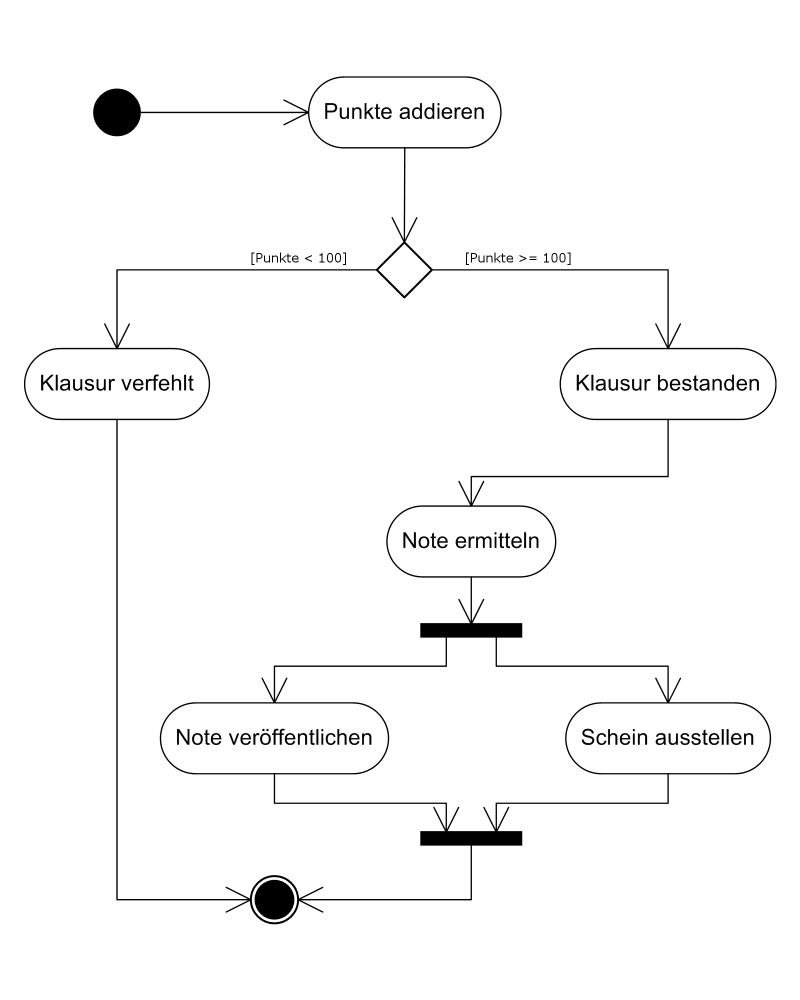
\includegraphics[scale=0.22]{pics/beispiel.png}
\end{center}
\end{exampleblock}
}

\frame{
\begin{center}
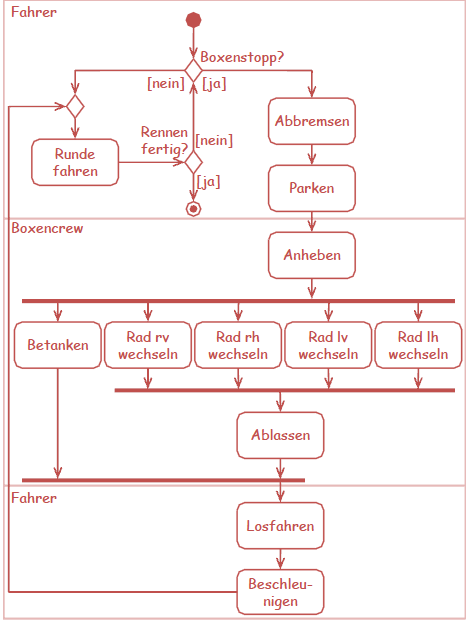
\includegraphics[scale=0.5]{pics/diagramm.png}
\end{center}
}

\section{Ende}

\subsection{Tipps zum nächsten Übungsblatt}

\frame{
\frametitle{Tipps zum nächsten Übungsblatt}

\begin{block}{Aufgabe 1 - Sequenzdiagramm}
\begin{itemize}
\item denkt an Attribute, Multiplizitäten, Restriktionen, Assoziationsnamen sowie Rollen \pause
\item merkt euch den Unterschied zwischen Komposition und Aggregation!
\end{itemize}
\end{block}

\begin{block}{Aufgabe 2 - Aktivitätsdiagramm}
\begin{itemize} \pause
\item ihr dürft die Aufgabe auf zwei Diagramme verteilen \pause
\item \url{http://de.wikipedia.org/wiki/Floyd-Steinberg-Algorithmus}
\end{itemize}
\end{block}

}


\frame{
\frametitle{Tipps zum nächsten Übungsblatt}
\begin{block}{Aufgabe 3 - Programmieren}
\begin{itemize}
\item args4j kann euch sehr viel Arbeit ersparen, versucht die Bedienung anhand von Configuration.java zu verstehen 
\item achtet darauf ob ihr Ganzzahldivision verwendet: 
\\ \pause
\texttt{int o; \dots; int p = (o + 128 ) / 256 * 255 \\
		// liefert hier 0 oder 255: wieso?}
\end{itemize}
\end{block}
}


\frame{
\frametitle{Bis zum nächsten Mal}
\begin{center}
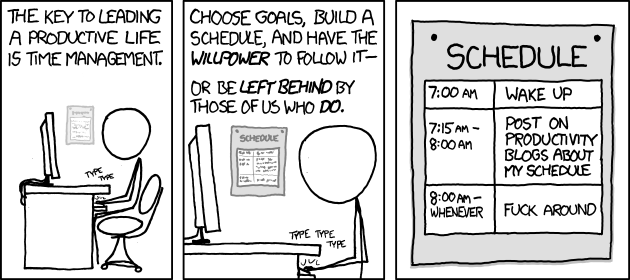
\includegraphics[width=1\textwidth]{pics/time_management}
\end{center}

}


\end{document}
